 
\documentclass[11pt,twoside,a4paper]{article}

\usepackage{graphicx}
\usepackage{epstopdf}

\begin{document}

\title{An example conjunctive water-energy nexus system using Pywr}
\author{James E. Tomlinson}
\date{December 2017}
\maketitle

\section{Introduction}

This short technical note summarises one approach to constructing a conjunctively operated energy-water system simulator. The purpose of this work was to create a minimum viable product (MVP) using existing Open Source software. The example seeks to demonstrate the following:

\begin{itemize}
    \item A true multi-resource multi-sector conjunctive use simulation model. That is a single simulator using a common algorithm to allocate multiple resource types across an interconnected network. 
    \item Conjunctive operation of multi-resource storage components. In most resource systems the operation of storage components (e.g. reservoirs, groundwater resource, batteries) is critical and causes most of the non-linearity. Typical operations must trade-off between utilising stored resource today or saving it for tomorrow. Here we seek to demonstrate conjunctively operating two storage components each storing a different resource.

\end{itemize}

\section{Example water-energy system}

The analysis in this technical note is based on a very simple multi-resource example. Figure \ref{fig:schematic} shows the example system. The components of this system are described below:

\begin{figure}
    \centering
    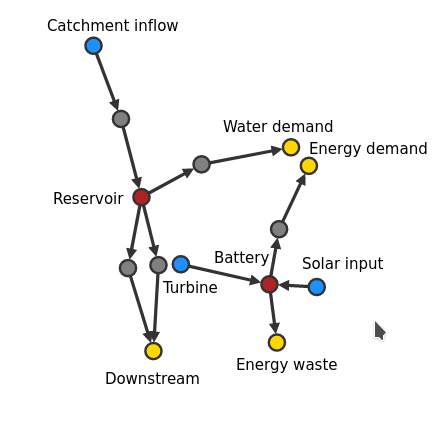
\includegraphics{schematic.png}
    \caption{A schematic of an example multi-resource network.}
    \label{fig:schematic}
\end{figure}

\begin{description}
    \item[Catchment] The single water inflow to the water part of the system. 
    \item[Reservoir] A water storage component. This component tries to keep itself as full as possible while meeting demands from both water demand centre and turbine. 
    \item[Water demand] A simple water demand centre requesting 3.0 $Mm^3$/day.
    \item[Turbine] The turbine is the primary interconnectivity between the water and energy networks. By default the turbine is limited to 1.0 $Mm^3$/day. Any flow through the turbine generates energy in the adjacent input node in the energy network. This is a simple fixed head relationship where $E(t) = q(t)\rho gh$. 
    \item[Solar] Solar input to the energy network is controlled by a timeseries of direct radiation [$MWh/m^2$/day]. The solar boundary condition defines a PV efficiency (20\%) and area (500,000 $m^2$). 
    \item[Battery] A energy storage component. By default this component is zero sized and represents a system with no ability to store energy. Similar to the water storage component the battery, when non-zero sized, attempts to keep itself as full as possible while meeting demands and balancing operation of the turbine.
    \item[Energy waste] Any unused energy (i.e. from solar) is tracked in this node. A key performance metric of the system is the total wasted energy. 
    \item[Energy demand] A simple energy demand centre requesting 125.0 $MWh$/day.
\end{description}

\subsection{Boundary conditions}

This simple example only requires two dynamic bounday conditiions: catchment inflow and direct radiation. Both are taken from a run of the UKCP09 weather generator at Oxford. The output is a daily timeseries of weather variables including rainfall and direct radiation. The rainfall timeseries is run through a simple monthly regression flow model for the river Thames. The flow and direct radiation timeseries are then both input as dynamic boundary conditions to Pywr. 

\subsection{Portfolios}

To illustrate some of the benefits of fast multi-resource simulation the example model has been setup with four portfolios. These portfolios modify different parameters in the model to represent different interventions that could be undertaken. The parameters altered are list in table \ref{tbl:portfolios}. 


\begin{table}
\begin{tabular}{ | c | c | c | c | }
\hline
Portfolio & Turbine capacity & Battery capacity  & Reservoir capacity \\
 &   [$Mm^3$/day] & [$MWh$] &  [$Mm^3$] \\
\hline
1 & 1.0 & 0.0     & 300 \\
2 & 1.0 & 0.5e3 & 300 \\
3 & 2.0 & 1.0e3 & 300 \\
4 & 2.0 & 1.0e3 & 400 \\
\hline
\end{tabular}
\caption{Portfolio setup}
\label{tbl:portfolios}
\end{table}

\section{Results}

The multi-resource simulator has been run through a 20 year simulation at a daily time-step for all portfolios. This run only takes a few seconds and produces some performance metrics while saving the timeseries of resource flux through each node. The performance metrics for the 4 portfolios are listed in table \ref{tbl:metrics}. Figures \ref{fig:water_timeseries} and \ref{fig:energy_timeseries} show the predicted timeseries for the important nodes in the water and energy sub-networks respectively. 

\begin{table}
\begin{tabular}{| c | c | c | c | c |}
\hline
Portfolio & 1 & 2 & 3 & 4 \\
\hline
Proportion of days with water deficit [\%] & 0.0 & 0.0 & 0.0 & 0.0 \\
Porportion of days with energy deficit [\%] & 0.604 & 0.309 & 0.004 & 0.000 \\
Total energy waste [$GWh$] & 535 & 446 & 473 & 478 \\
\hline
\end{tabular}
\caption{Example performance metrics}
\label{tbl:metrics}
\end{table}

An important observation is the balancing of the two storage components. The dynamic allocation routine seeks to operate the turbine to keep the relative current storage at a similar position in both the reservoir and the battery.


\begin{figure}
    \centering
    \includegraphics[width=\linewidth]{../outputs/figures/catchment1.png}
    \includegraphics[width=\linewidth]{../outputs/figures/turbine1.png}
    \includegraphics[width=\linewidth]{../outputs/figures/reservoir1.png}
    \includegraphics[width=\linewidth]{../outputs/figures/water_demand1.png}
    \caption{Simulated timeseries for water nodes.}
    \label{fig:water_timeseries}
\end{figure}

\begin{figure}
    \centering
    \includegraphics[width=\linewidth]{../outputs/figures/solar1.png}
    \includegraphics[width=\linewidth]{../outputs/figures/turbine_generator1.png}
    \includegraphics[width=\linewidth]{../outputs/figures/battery1.png}
    \includegraphics[width=\linewidth]{../outputs/figures/energy_waste1.png}
    \caption{Simulated timeseries for energy nodes.}
    \label{fig:energy_timeseries}
\end{figure}



\section{Conclusion}

This technical note is a very simple example of a multi-resource network simulation. It is only one approach to this problem, and has been developed from a background of water resource modelling. It is worth discussing the technical merits and drawbacks of using such an approach in a complex real world system.

\end{document}
